\chapter{Coulomb explosion imaging}\label{ch:CEI}

\vspace{-1.5 em}
\begin{addmargin}[-0.5cm]{0cm}
  \minitoc
\end{addmargin}
\hrule
\vspace{1.5 em}

\section{What's the deal with Coulomb explosion imaging?}
What is Coulomb explosion imaging? A technical definition could be given, however, it is simply a decades-old technique in a long line of techniques stretching back centuries, all meant to answer a question posed by the ancient Greeks and Indians---what are the building blocks of the universe, and how do they behave?

It is easy to get stuck in the ivory tower and get lost within the trees of science, losing sight of the big picture of where your research leads.

\pagebreak
\begin{figure}
  \centering
  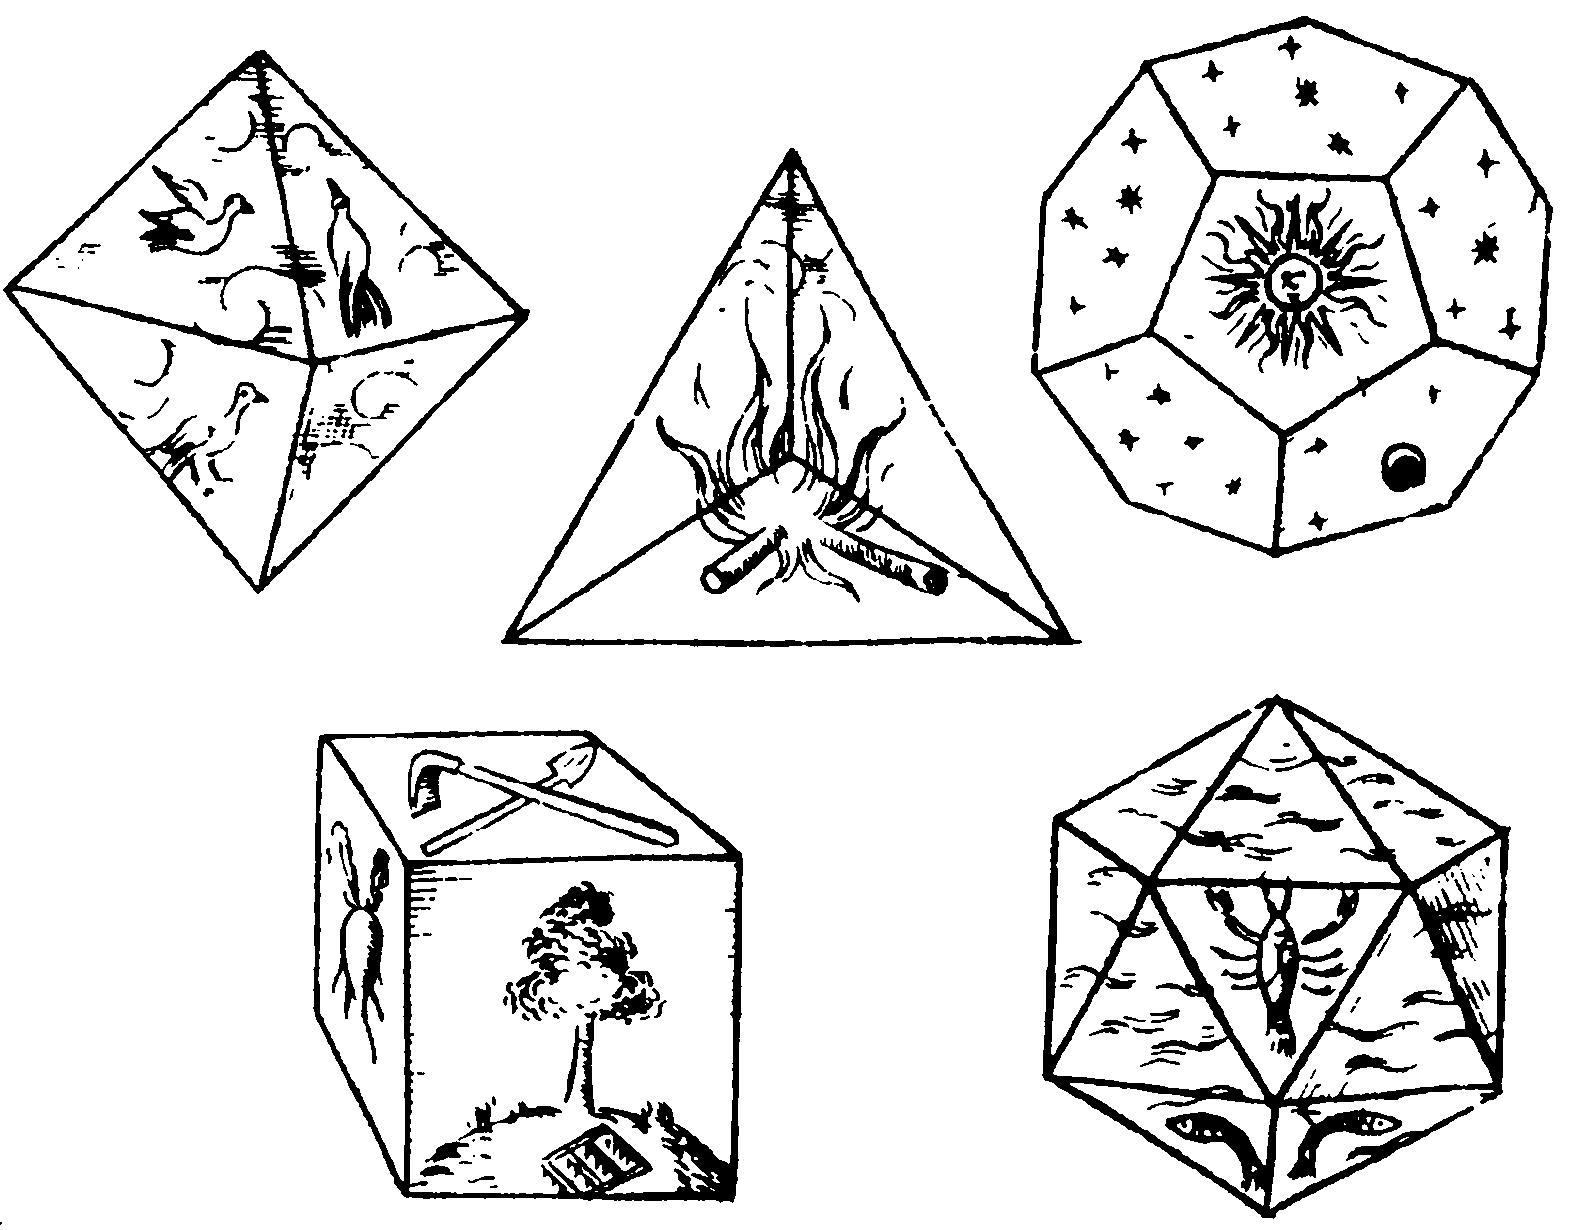
\includegraphics[width=\textwidth]{gfx/PlatonicSolids}
  \caption[The classical elements associated with the five Platonic solids.]
  {The classical elements associated with the five Platonic solids. Clockwise from the top left: the octahedron with air, tetrahedron with fire, dodecahedron with the universe, the isocehedron with water, and the cube with earth. Figure from \citet[Book 2, p. 53]{Kepler1619}. English translation available \citep{Kepler97}.}
  \label{fig:platonicSolids}
\end{figure}
\clearpage

\section{Physical principles and experimental outline}\label{sec:CEIphysics}

%\subsection{Pump-probe Coulomb explosion imaging}
In pump-probe Coulomb explosion imaging (CEI) one ultrashort laser pulse is split into two pulses through the use an asymmetric beamsplitter. One of the pulses, the pump pulse, is usually much weaker than the other, the probe pulse. A time delay $\tau$ between the pulses is then created such that the pump pulse goes first and the probe pulse second. The job of the pump pulse will be to initiate some change in the molecule. One example could include an isomerization of the molecule. Thus the pump pulse ``pumps'' the molecule into some excited state. The job of the powerful probe pulse is to engulf the molecule in an intense enough laser field such that multiple electrons are stripped off of it. The molecule's individual atoms are left in a highly-charged state and begin to behave as individual point charges in a purely Coulombic potential. The entire process occurs in the presence of a constant electric field and so the positively-charged ions all accelerate upwards towards a time- and position-sensitive detector. Thus the probe pulse allows for the ``probing'' of the excited state.

%\subsection{Femtosecond Multiple Pulse Length Spectroscopy}

\section{History of molecular geometries seen using Coulomb explosion imaging}
The original CEI experiment is usually traced back to \citet{Vager89} in which the Coulomb explosion is initiated by passing a molecular beam through a thin foil. This may be because it was the first work suggesting that full molecular structures may be recovered by measuring the velocity (or momentum) vectors of the atomic fragments, and even reported on a non-classical molecular structure. However, previous works utilizing CEI do exist, even some significant works that report on molecular structures \citep{Kanter79}.

Ultrashort laser pulses\footnotemark as a means of inducing Coulomb explosions made their entrance in the 1980's where they were utilized to infer molecular dynamics using covariance mapping \citep{Frasinski89}. Highly charged ion impact is another method of inducing a Coulomb explosion, and was first done in the 1990's in parallel with the development of more sophisticated coincidence mapping techniques. Since then, the laser has emerged as the more popular tool and has further developed the coincidence mapping technique. There do exist other methods of inducing Coulomb explosions, for example, single photons from a synchrotron source utilizing the Auger effect, x-ray pulses from a free-electron laser source, or electron collision.

\footnotetext{In 1987, ultrashort would be referring to \SI{0.6}{\pico\s} laser pulses \citep{Frasinski87}.}

In this section we will trace the history of CEI back to the 1970's where it started with foil-induced fragmentation. We will then follow it's development to the present day where ultrashort laser pulses are the most popular means of performing CEI. Throughout we will focus solely on the achievements of CEI in determining molecular structures, and in creating molecular movies using these recovered structures.\footnotemark

\footnotetext{Much of the molecular dynamics are inferred in CEI from studying the distribution of the fragment momentum vectors (\eg through the use of Newton and Dalitz plots) and the distribution of kinetic energy carried away by each fragment. We will be focusing on the original aim of CEI, that is, to measure molecular structures.}

Interestingly, the first-ever mention of the term ``Coulomb explosion'' in the published literature comes from an unrelated study of the fine structure of singly ionized helium by \citet{Novick55}. They measured the energy difference of the $2 \, ^2 S_{1/2}$ and $2 \, ^2 P_{1/2}$ states of ionized helium as a sensitive test of quantum electrodynamics. Coulomb explosion (or space charge explosion) was the dominant ion removal mechanism which they accounted for in modeling the quenching rate\footnotemark of metastable $2 \, ^2 S_{1/2}$ ions by radio frequency radiation to describe the observed resonance lineshapes (spending two appendices on it).

\footnotetext{The term was more popular in decades past but simply means the extinction rate or loss rate of metastable ions.}

\subsection{Foil-induced dissociation}
CEI was first performed by passing a molecular beam containing the molecule of interest through a thin atomic film. Figure \ref{fig:foilExperiment} shows a schematic of such an experiment. While in the solid film, the probability for Coulomb scattering of the individual atomic nuclei is small due to their small size and consequently small interaction cross-section. However, the electrons will be scattered to very wide angles due to their interaction with the many electron clouds in the film. This process rapidly ionizes the molecule, typically within the first few atomic layers or the first femtosecond. The now highly ionized molecule exits the foil and rapidly dissociates into its consituent atomic fragments which repel eachother under their mutual Coulomb repulsion in what is termed a ``Coulomb explosion''.

\begin{figure}[H]
  \centering
  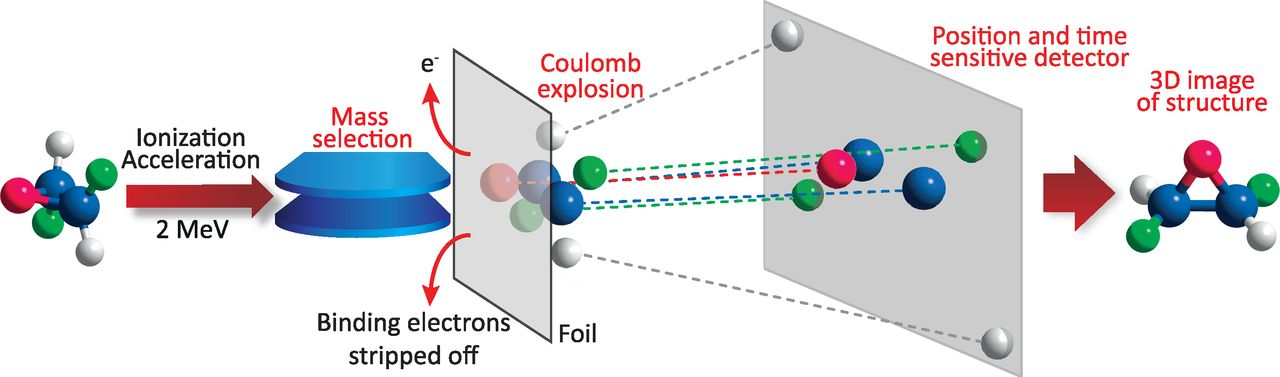
\includegraphics[width=\textwidth]{gfx/FoilExperiment}
  \caption[Schematic of a foil-induced Coulomb explosion imaging experiment.]
  {Schematic of a foil-induced Coulomb explosion imaging experiment. This specific experiment set out to measure the absolute configuration of atoms in a chiral molecule in the gas phase, which remains challenging. Early foil-induced CEI experiments can be described by this schematic except for the fact that they did not employ a mass selector and used a more primitive but still position-sensitive detector. The atomic fragment trajectories (dashed lines) assume that no rearrangement of the atoms occurs and that the system evolves under a Coulomb potential. From \citet{Herwig13}. Reprinted with permission from AAAS.}
  \label{fig:foilExperiment}
\end{figure}

The premise behind foil-induced CEI is that during this explosion, the atoms simply repel each other and do not rearrange, thus preserving the angles between them from the time they exit the foil to the time they are detected at a position and time-sensitive detector. As the potential energy of each pair of fragments $i,j$ is coverted to kinetic energy according to
\begin{equation}\label{eq:foilCEI}
\frac{4q_i q_j}{|\mathbf{r}_i - \mathbf{r}_j|} = \frac{\mu|\mathbf{V}_i - \mathbf{V}_j|^2}{2}
\end{equation}
it suggests that measurement of the asymptotic vector velocities completely defines the initial geometry of the molecule \citep{Vager89}. Here $q_i$, $\mathbf{r}_i$, and $\mathbf{V}_i$ are the charge, position vector, and velocity vector of the atomic fragment $i$ while $\mu$ is the reduced mass of the two-body system of fragments $i,j$.

\begin{figure}[H]
  \centering
  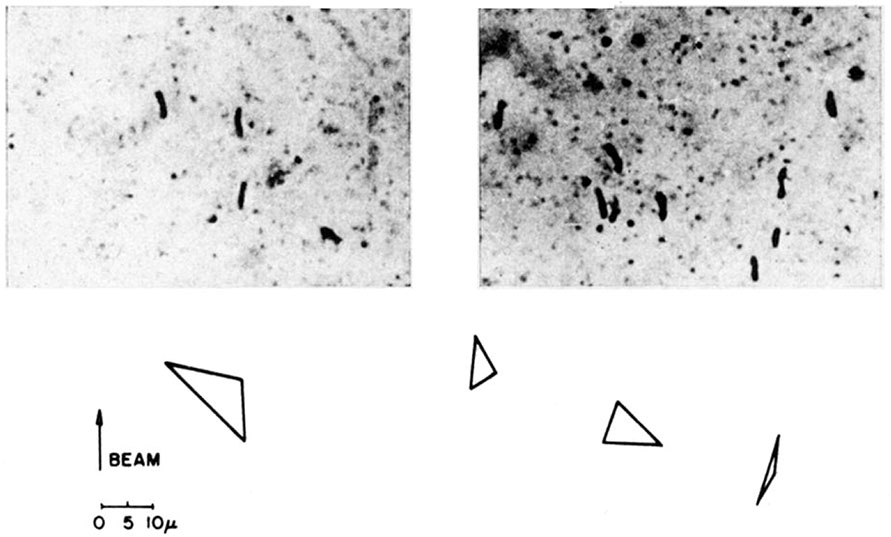
\includegraphics[width=\textwidth]{gfx/HydrogenTrimerReconstruction}
  \caption[Reconstructions of exploded \ch{H3+} following foil-induced dissociation.]
  {Reconstructions of exploded \ch{H3+} following foil-induced dissociation. On the top row are a couple of good photographs of exploded \ch{H3+} recorded on photographic emulsion at a tilt angle of $30\degree$. The bottom row shows a few reconstructions (normally projected) made by inspection from the photographs. The authors analyzed 350 such photographs and concluded that \ch{H3+} mainly exhibits an equalateral triangle geometry. From \citet{Gaillard78}. Reprinted with permission from APS.}
  \label{fig:hydrogenTrimer}
\end{figure}

The earliest example of a molecular geometry recovered using CEI is reported by \citet{Gaillard78}. They used the foil-induced Coulomb explosion to image the structure of the \ch{H3+} molecular ion, showing that it is mainly exhibits an equalaterial triangular shape in three completely different experiments.\footnotemark ~Figure \ref{fig:hydrogenTrimer} gives a few examples of the geometries they recovered.

\footnotetext{It is interesting to note that the experiment was repeated by three separate teams, then reported on coherently in one manuscript. Each team, having access to different equipment, produced separate pieces of data. It was the team in Rehovot, Israel that recorded the projections of the exploded ions while the others measured energy spectra and angular distributions.}

It is unclear how the idea for such an imaging experiment came to be, however it worth noting that \citet{Gaillard78} and co-authors have been studying the effects of molecular beams passing through thin foils for quite some time, mainly at Argonne National Laboratory. See for example their studies of wake potentials generated behind charged particles as they pass through a solid \citep{Gemmell75, Vager76PRL} and their study of the dissociation of fast \ch{HeH+} ions traversing thin foils \citep{Vager76PRA}. It seems quite reasonable that studying the dissociation of small molecules and the angular distribution of the fragments would inspire researchers to attempt to infer molecular structures using this data.

A more popular CEI experiment was performed by \citet{Vager89} almost a decade later employing a $\sim$\SI{30}{\angstrom} aluminum film. Their work was motivated by the opportunity of imaging non-classical molecular structures that more popular methods were incapble of seeing. They were also the first to suggest that measuring the velocity (or momentum) vectors of each fragment would be provide all the information required to describe the molecule's structure. Figure \ref{fig:C2H3geometry} shows one reconstruction based on the measured velocity vectors.

\begin{figure}
  \centering
  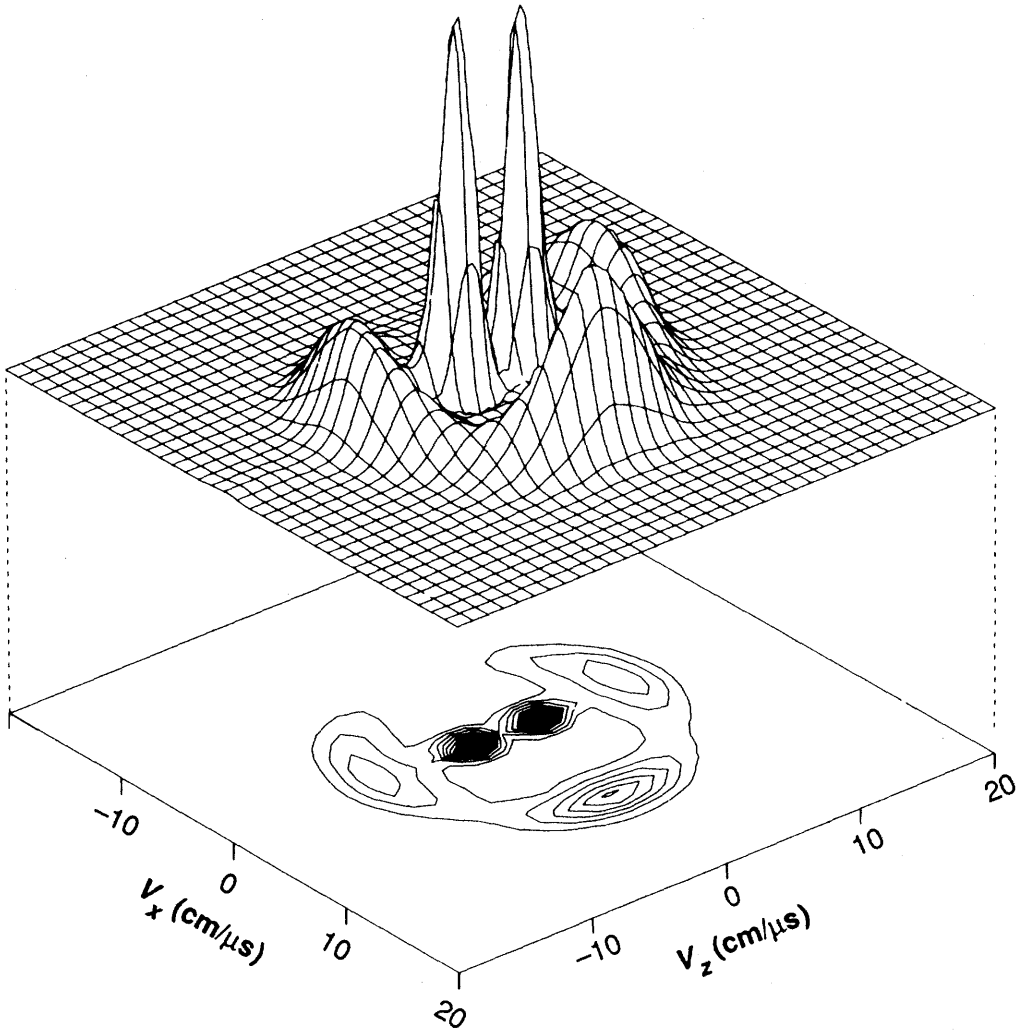
\includegraphics[width=\textwidth]{gfx/VagerPseudoGeometry}
  \caption[Reconstruction of \ch{C2H3+} following foil-induced dissociation.]
  {Reconstruction of \ch{C2H3+} following foil-induced dissociation. The densities of the fragment ions are plotted in a coordinate system defined by the final velocities of each particle (relative to the mean carbon-ion velocity). Assuming \eqref{eq:foilCEI} holds, this is an inference of the geometry, and quite a convincingly pretty one at that. The carbon ion densities were reduced by a factor of $5$ for display purposes. From \citet{Vager89}. Reprinted with permission from AAAS.}
  \label{fig:C2H3geometry}
\end{figure}

However, they do not perform any geometry reconstruction and report their fragment ion densities in a coordinate system defined by the asymptotic velocity of each particle, and claim that it is a direct measurement of the square of the multidimensional wave function of a many-body system.

The promise of recovering molecular geometries in this simple fashion seems quite empty after glancing at the published literature in the past few decades. While foil-induced CEI has found some uses and produced some interesting work in recent years\footnotemark~, for the purposes of studying molecular structures and dynamics, the ultrafast laser shortly thereafter became the tool of choice for CEI as we will discuss in section \ref{sec:laserCEI}. The reason for the scarcity of foil-induced CEI experiments in the published literature is mainly due to its limitations.

\footnotetext{This includes imaging the rovibrational wave functions of \ch{H2-} and \ch{D2-} by studying the kinetic energy relased by the fragments \citep{Jordon-Thaden11, Herwig13PRA}, and imaging the absolute configuration of chiral molecules in the gas phase by studying the measured velocity vectors of the fragments with Newton plots \citep{Herwig13}.}

Of course, there are some assumptions that must hold for a complete and accurate recovery of the initial geometry, which we shall discuss in section \ref{sec:CEIphysics}. However, just by inspection of the schematic in figure \ref{fig:foilExperiment} we can see that no rearrangement of the atoms must occur\footnotemark~ and that the molecular system must evolve on the Coulomb potential, which requires the rapid stripping of many electrons off the atom. Thus CEI becomes increasingly difficult to perform with larger molecules so it is best used to study smaller molecules. However, it is precisely these small molecules in the gas phase that need to be studied using CEI as they cannot be probed using other more established methods. Moreover, many smaller molecules may exhibit non-Coulombic behaviour unless placed into a highly charged state, which may be impossible depending on the apparatus in use. For foil-induced CEI in particular, a molecular beam must be prepared, and this may prohibit the study of many molecules that cannot be prepared as such.

\footnotetext{While this is the case for many smaller molecules, it is not true for some of the popular targets. For example, a triatomic molecule may dissociate into a single atom and a diatomic rotor, which rotates before dissociating into two atoms.}

\subsection{Imaging with ultrashort laser pulses}\label{sec:laserCEI}

\subsubsection*{Attempt at an analytical solution}
\index{Classical imaging formula}
\index{Coulomb explosion imaging!Classical imaging formula}
Before taking a tour of the molecular geometries recovered using laser-induced CEI, it is worth mentioning that \citet{Nagaya04} have attempted to arrive at an analytical solution for calculating molecular geometries from measured momentum vectors. They were able to derive a ``classical imaging formula''
\begin{equation}
|\Psi_\mathrm{image}(R_I)|^2 = S(p) \frac{1}{P_\mathrm{ion}(R_I)} \sqrt{\frac{\mu q_A q_B}{8\pi\epsilon_0 R_I^3}} , \quad R_I = \frac{\mu q_A q_B}{2\pi\epsilon_0 p^2}
\end{equation}
where
\begin{equation}
S(p) = |c(p)|^2 = \left| \int \Phi_C^*(p,r) T_\mathrm{ion}(r) \Psi(r) \; dr  \right|^2
\end{equation}
for the position wavefunction of a molecule in terms of its momentum distribution $S(p)$. They are able to derive a similar formula for the Coulomb explosion of a symmetric linear triatomic molecule, but the more general case of the asymmetric linear triatomic molecule proves much more formidable.\footnotemark ~They proceed to compare their ``classical'' reconstructions for the vibrational wavefunction of a helium trimer system to the predictions of the quantum theory, noting small discrepencies. The bulk of their article focuses on the Coulomb explosion of asymmetric linear triatmoic molecules and derives a two-dimensional classical imaging formula in terms of hyperspherical coordinates. An extension to three dimensions for bent triatomic molecules is promised but could not be found in the published literature.

\footnotetext{While a highly commendable effort, their unsaid conclusion seems to be that this is an intractable problem as their research group seems to have gone silent on this problem and the only citations to this work are in the context of the difficulty of the problem.}

\subsubsection*{Inferring dynamics from energy spectra and momentum vector distribtuions}
Due to the difficulty of recovering the molecular geometries, the structures and dynamics of small molecules are usually inferred from the kinetic energy spectra of the fragments and their momentum vector distributions (usually studied using Newton and Dalitz plots).

\subsubsection*{Experimental reconstructions}
\citet{Legare05structure,Legare05dynamics} were the first to use ultrashort laser pulses (\SI{8}{\fs}) and CEI to report on molecular structures and dynamics. Figure \ref{fig:SO2-232structure} shows a reconstruction of \ch{SO2} using the \ch{SO2^{7+}} charge state. To obtain the structures, they assume the explosion system evolves under a purely Coulombic potential and use optimization methods to make guesses at the structure that most accurately reproduces the observed data consistent with minimizing a least-squares objective function. Treating the geometry reconstruction as an optimization problem is exactly what we do in chapter \ref{ch:optimization}. However, dissapointly, they trivialize the solution to a couple of sentences and fail to report the optimization methods employed, sidestepping the nuances of the reconstruction process that we will discuss in chapters \ref{ch:lookupTable}--\ref{ch:bayesian}. The nuances include the existence, in some cases, of multiple molecular structures producing the same momentum vector distribution (dubbed degenerate geometries) and the high sensitivity of the reconstructed initial geometry to uncertainties in the momentum vectors leading to very uncertain geometries in some cases. Without knowledge of the optimization methods used, it is impossible to tell whether appropriate methods were used. We will show that this is an ill-posed inverse problem, or rather, a constrained nonlinear optimization problem calling for optimization methods that are typically outside the scope of introductory optimization textbooks.

\begin{figure}
  \centering
  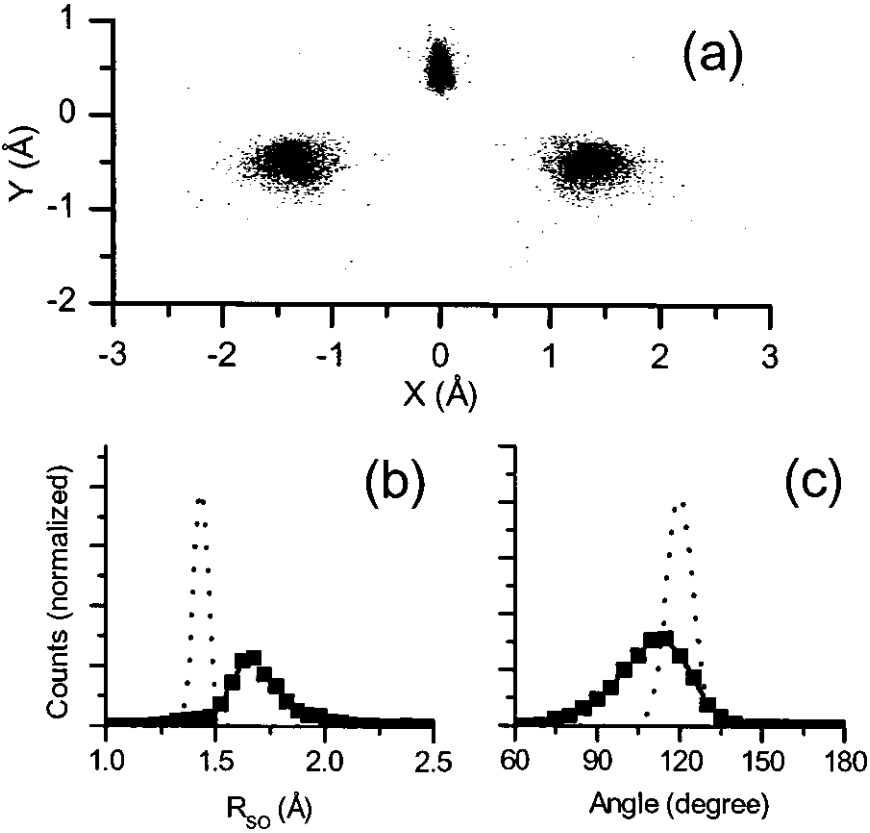
\includegraphics[width=\textwidth]{gfx/LegareSO2-232Structure}
  \caption
  [Molecular structure of \ch{SO2} using the \ch{SO2^7+} charge state.]
  {(a) Molecular structure of \ch{SO2} using the \ch{SO2^7+} charge state (\ch{SO2^7+ $\rightarrow$ O^2+ + S^3+ + O^2+}). The center of mass is at $x=0$, $y=0$, and the $y$-axis is the bisector of the angle. While an intuitive way to plot geometries, we will show that such a plot can hide unphysical correlations in the reconstructed geometries. (b) Radial distribution and (c) angular distribution of the reconstructed geometries with the dotted lines showing the expected distributions for the $\nu=0$ stationary state structure of \ch{SO2}. While the results again make intuitive sense, it would be interesting to see whether the radial distributions of both bond lengths to help ascertain the robustness of their reconstruction method. These marginal distributions are typically of the greatest interest but we will show that they can be used to hide unphysical correlations, and that joint distributions should be reported. From \citet{Legare05structure}. Reprinted with permission from APS.}
  \label{fig:SO2-232structure}
\end{figure}

They also claim to have imaged vibrating \ch{D2^+} and dissociating \ch{SO2^2+} and \ch{SO2^3+} however they provide no more than a couple of dissociation frames and infer the transient \ch{D2^+} bond length from kinetic energy release ratios as a function of pump-probe time delay \citep{Legare05dynamics}.

\citet{Gagnon08} reported the reconstruction of dichloromethane (\ch{CH2Cl2}) using a home-made \footnotemark stochastic-based simulated annealing algorithm that globally optimizes the molecular spatial configuration. They discuss uncertainties but are only able to obtain the structure in five cases.

\footnotetext{There is nothing wrong with writing your own code here but nonconvex optimization algorithms are tricky to get right and professional optimization libraries (both proprietary and open-source) do exist. At least the methods and source code are publicly available \citep{Gagnon06}.}

\begin{SCfigure}
  \centering
  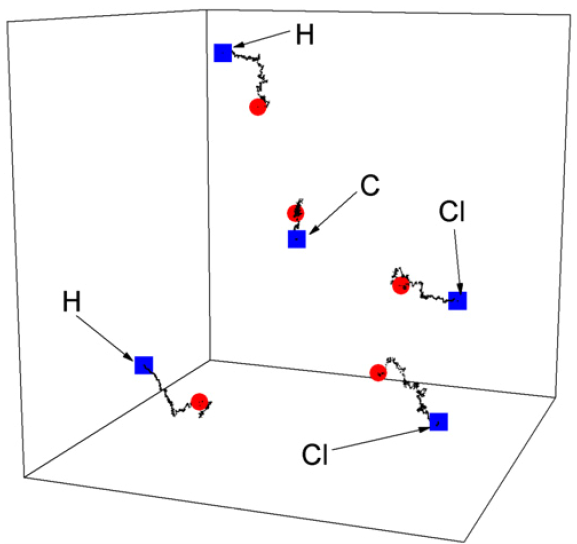
\includegraphics[width=0.5\textwidth]{gfx/CH2Cl2Geometry}
  \caption
  [Geometry of \ch{CH2Cl2}.]
  {Geometry of \ch{CH2Cl2}. From \citet{Gagnon08}. Reprinted with permission from IOP.}
  \label{fig:CH2Cl2geometry}
\end{SCfigure}

\index{Lookup table}
The best geometry reconstruction effort so far has is most likely the imaging of the Efimov state of the helium trimer by \citet{Kunitski15}, coming full circle to the very first images of the hydrogen trimer \citep{Gaillard78}.

% Purpose: Audience can discuss why methods other than foil and laser aren't so good for imaging molecular geometries.
% \subsection{Other methods of inducing Coulomb explosions}

\subsection{Molecular movies}
Molecular movies are of course not only of interest in physics and chemistry as a means of probing fundamental processes, but also in the biological sciences where molecular structure play a crucial role in determining the function of biomolecules such as proteins. However, the molecules of interest there are much too large to be studied by any of the previous techniques. Thus molecular movies in the biological sciences tend to be annotated computer simulations amalgamated from multiple studies. That said, they are very impressive pieces of work.

A particularly impressive movie by \citet{Cheung12} showcases the process of RNA polymerase transcription and goes on for over six minutes.

\section{Data measurement and analysis}
The premise of CEI is simple enough for a quirky elevator pitch yet the collecton and analysis of data is a nuanced multi-step process as we are attempting to measure each single atomic fragment precisely. In this section we will go through the process of how the momentum vectors of each atomic fragment are measured. This will require some discussion regarding the apparatus, algorithms, and intricacies of the process, all of which are essential to understand exactly how the data is collected so that it can be analyzed appropriately. We will also quantify the uncertainty in those measurements, which will be essential in quantifying our uncertainty in the reconstructed geometries later on.

\subsection{Time and position measurement}
The time-of-flight of each atomic fragment and its position on the detector are required to calculate its momentum vector. The measurement of time and position is carried out by a two-stage apparatus feeding electrical signals into a data acquisition (DAQ) computer which analyzes the signals to determine time and position.

The first part of the two-stage apparatus is a set of two multi-channel plates (MCP) placed in a chevron configuration.\footnotemark~ Figure \ref{fig:MCP} shows a schematic of an MCP and briefly describes its operation. The job of the MCP is to amplify the signal of a single charged particle enough such that it may be detected as an electrical signal by an oscilloscope, much like a photomultiplier tube. Thus the output of an MCP is a shower of charged particles, or rather a charged cloud. The charged cloud may be fed into a second MCP to further amplify the signal. A two-stage chevron MCP setup produces an amplification of approximately $10^5-10^6$ depending on the applied voltage $V_D$ across the channels.

\footnotetext{The channels of an MCP are slanted, usually at a (bias) angle of $5\degree-15\degree$ to increase the probability that an incident particle collides with the channel wall. To further increase this probability, the second MCP is oriented such that its channels are slanted in the opposite direction forming a V-like (or chevron-like) channel configuration.}

\begin{SCfigure}
  \centering
  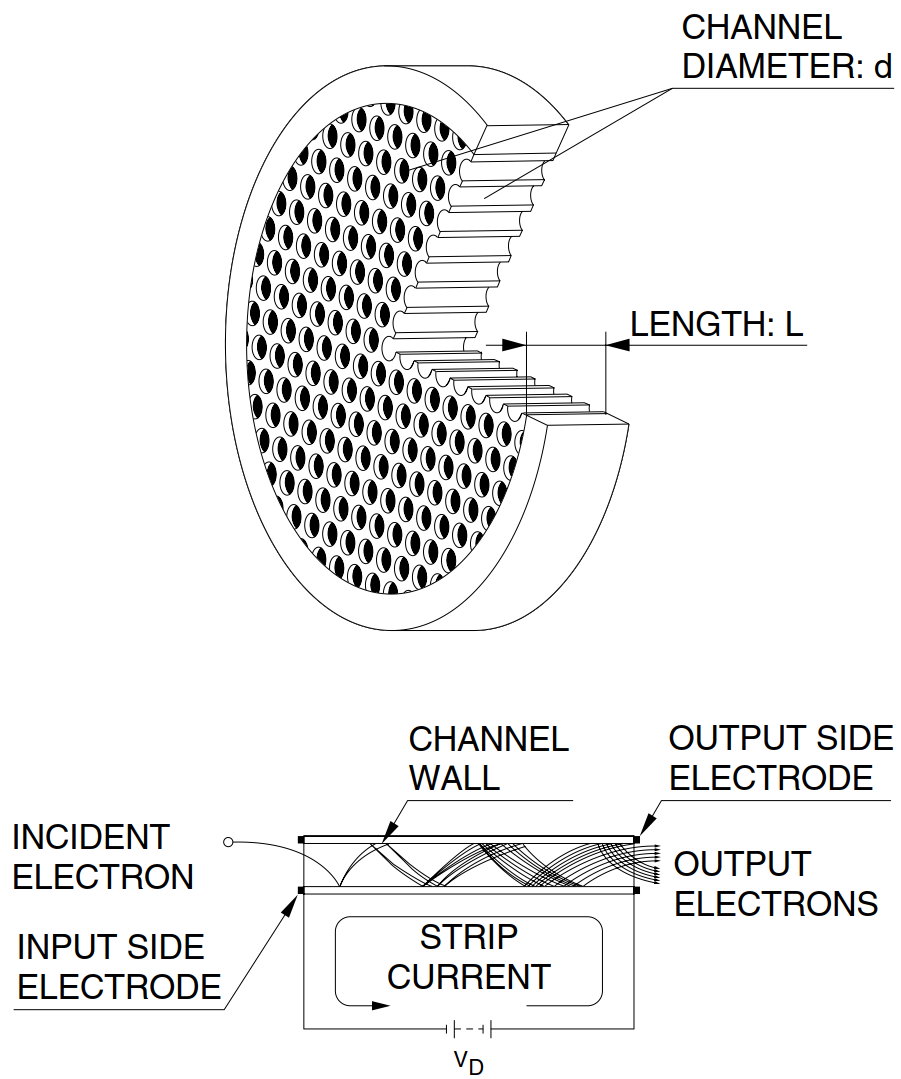
\includegraphics[width=0.50\textwidth]{gfx/MCP}
  \caption
  [Schematic of a multi-channel plate (MCP).]
  {Schematic of a multi-channel plate (MCP). The incident particle need not be an electron, and may in fact be any charged particle or even a high-energy photon. Once a charged particle is incident on an MCP and collides with a channel wall, multiple secondary electrons are emitted and accelerated up the channel due to the applied voltage $V_D$ setting up a potential gradient along the channel and replenishing the emitted electrons. Due to the angled channels, the emitted electrons follow parabolic trajectories hitting the other wall and continuing the amplification process until a large number of particles are emitted at channel output.}
  \label{fig:MCP}
\end{SCfigure}

You may notice that while most of the MCP's surface is covered in channels, not all of it is, leading to non-perfect detection. Only 60\% of the area is open to incident particles, and if a particle is incident on the other 40\% then it is not detected. Thus the detection efficiency of a triple coincidence event is $(0.6)^3 \approx 0.2$ and so we see that detection effiency decreases rapidly with the number of fragments that must be detected, suggesting that larger molecules are more difficult to study. There do exist ``funnel'' MCPs with an open area ratio of 90\% that increase the detection efficiency.

By itself this MCP setup is enough to provide time-of-flight information but to obtain position information, this charged cloud output is made incident on a ``modified backgammon with weighted capacitors'' anode or readout pad built as described by \citet{Veshapidze02}. Figure \ref{fig:MBWC} shows a schematic of such an anode and describes the position detection process.

\begin{figure}
  \centering
  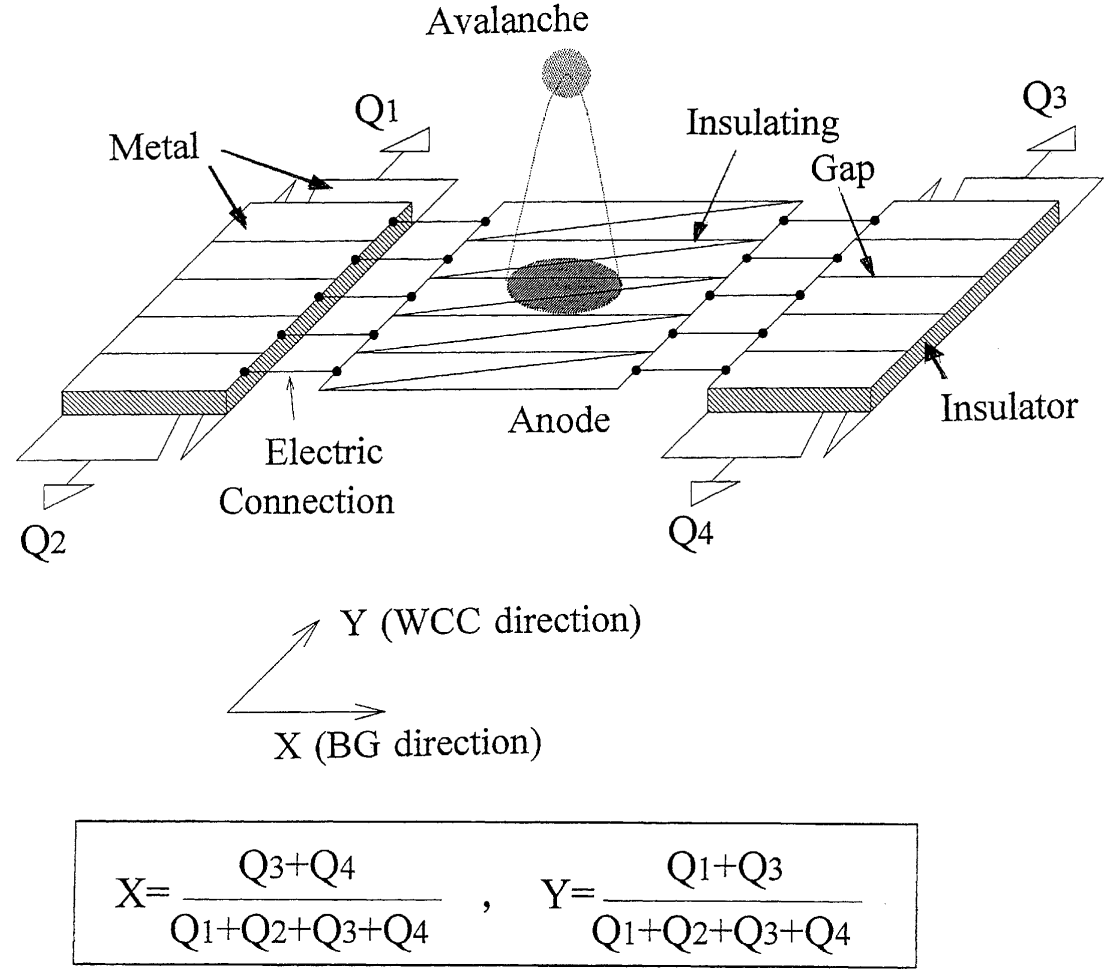
\includegraphics[width=\textwidth]{gfx/MBWC}
  \caption
  [Schematic of a symmetrized ``modified backgammon with weighted capacitors'' (MBWC) anode for position detection.]
  {Schematic of a symmetrized ``modified backgammon with weighted capacitors'' (MBWC) anode for position detection. The avalanche of charged particles or charged cloud hits the anode and induces a charge on the anode. This charged is induced via the capacitive couplings from the feedback capacitors of the preamplifiers connected to the triangles. The lines on the anode are insulating gaps, splitting the anode into a series of triangles whose arrangement resemble that of the backgammon board game. The metal strips are capacitively coupled to the triangluar strips through the insulator. If the cloud lands on the right side of the anode, then a larger fraction of the induced charge will flow to $Q_3$ and $Q_4$. So we can see that $x=0$ corresponds to the left side of the anode, and $x=1$ to the right side. If the cloud lands further up the anode, then a larger fraction of the induced charge will flow through $Q_1$ and $Q_3$ so we see that $y=0$ corresponds to the bottom side of the anode and $y=1$ corresponds to the top side. It is worth noting that the sign of $Q_i$ depends on the sign of the induced charge, and thus on the sign of the incident charged particle. In CEI the charged particles are all ions so $Q_i$ is always positive. The design gets its name as it is a combination of two older designs, the ``backgammon'' (BG) and the ``weighted coupling capacitor'' (WCC) designs. \citet{Mizogawa92} provides a more detailed explanation of its operation.  Figure rom \citet{Mizogawa02}. Reprinted with permission from Elsevier.}
  \label{fig:MBWC}
\end{figure}

These four signals are fed into an Ortec 142 preamplifier in energy output mode, essentially acting as an operational amplifier integrator. The integrated signal is then fed into a digital acquisition (DAQ) computer equipped with a four-channel oscilloscope. Every time a laser pulse is fired into the experiment, an electrical signal is sent to the oscilloscope as a trigger. The DAQ examines the four signals following a trigger and saves them if it sees evidence of charged particle detection.

A particularly good example of a triple coincidence detection event can be seen in figure \ref{fig:tripleCoincidence} along with an analysis of what can be gleaned about the Coulomb explosion process just by inspection of the signals on the oscilloscope. As a side note, if too many atomic fragments arrive at the detector in a short enough time period, steps due to different molecules may get mixed. Thus it is important to keep the Coulomb explosion rate low (\SI{100}{\Hz} worked quite well). Another reason to keep the count rate low is that the signals need time to decay back down post-integration otherwise the signals will saturate the oscilloscope at \SI{200}{\mV}. The ringing artifacts on the signal are due to the response of the preamplifiers.

\begin{figure}
  \centering
  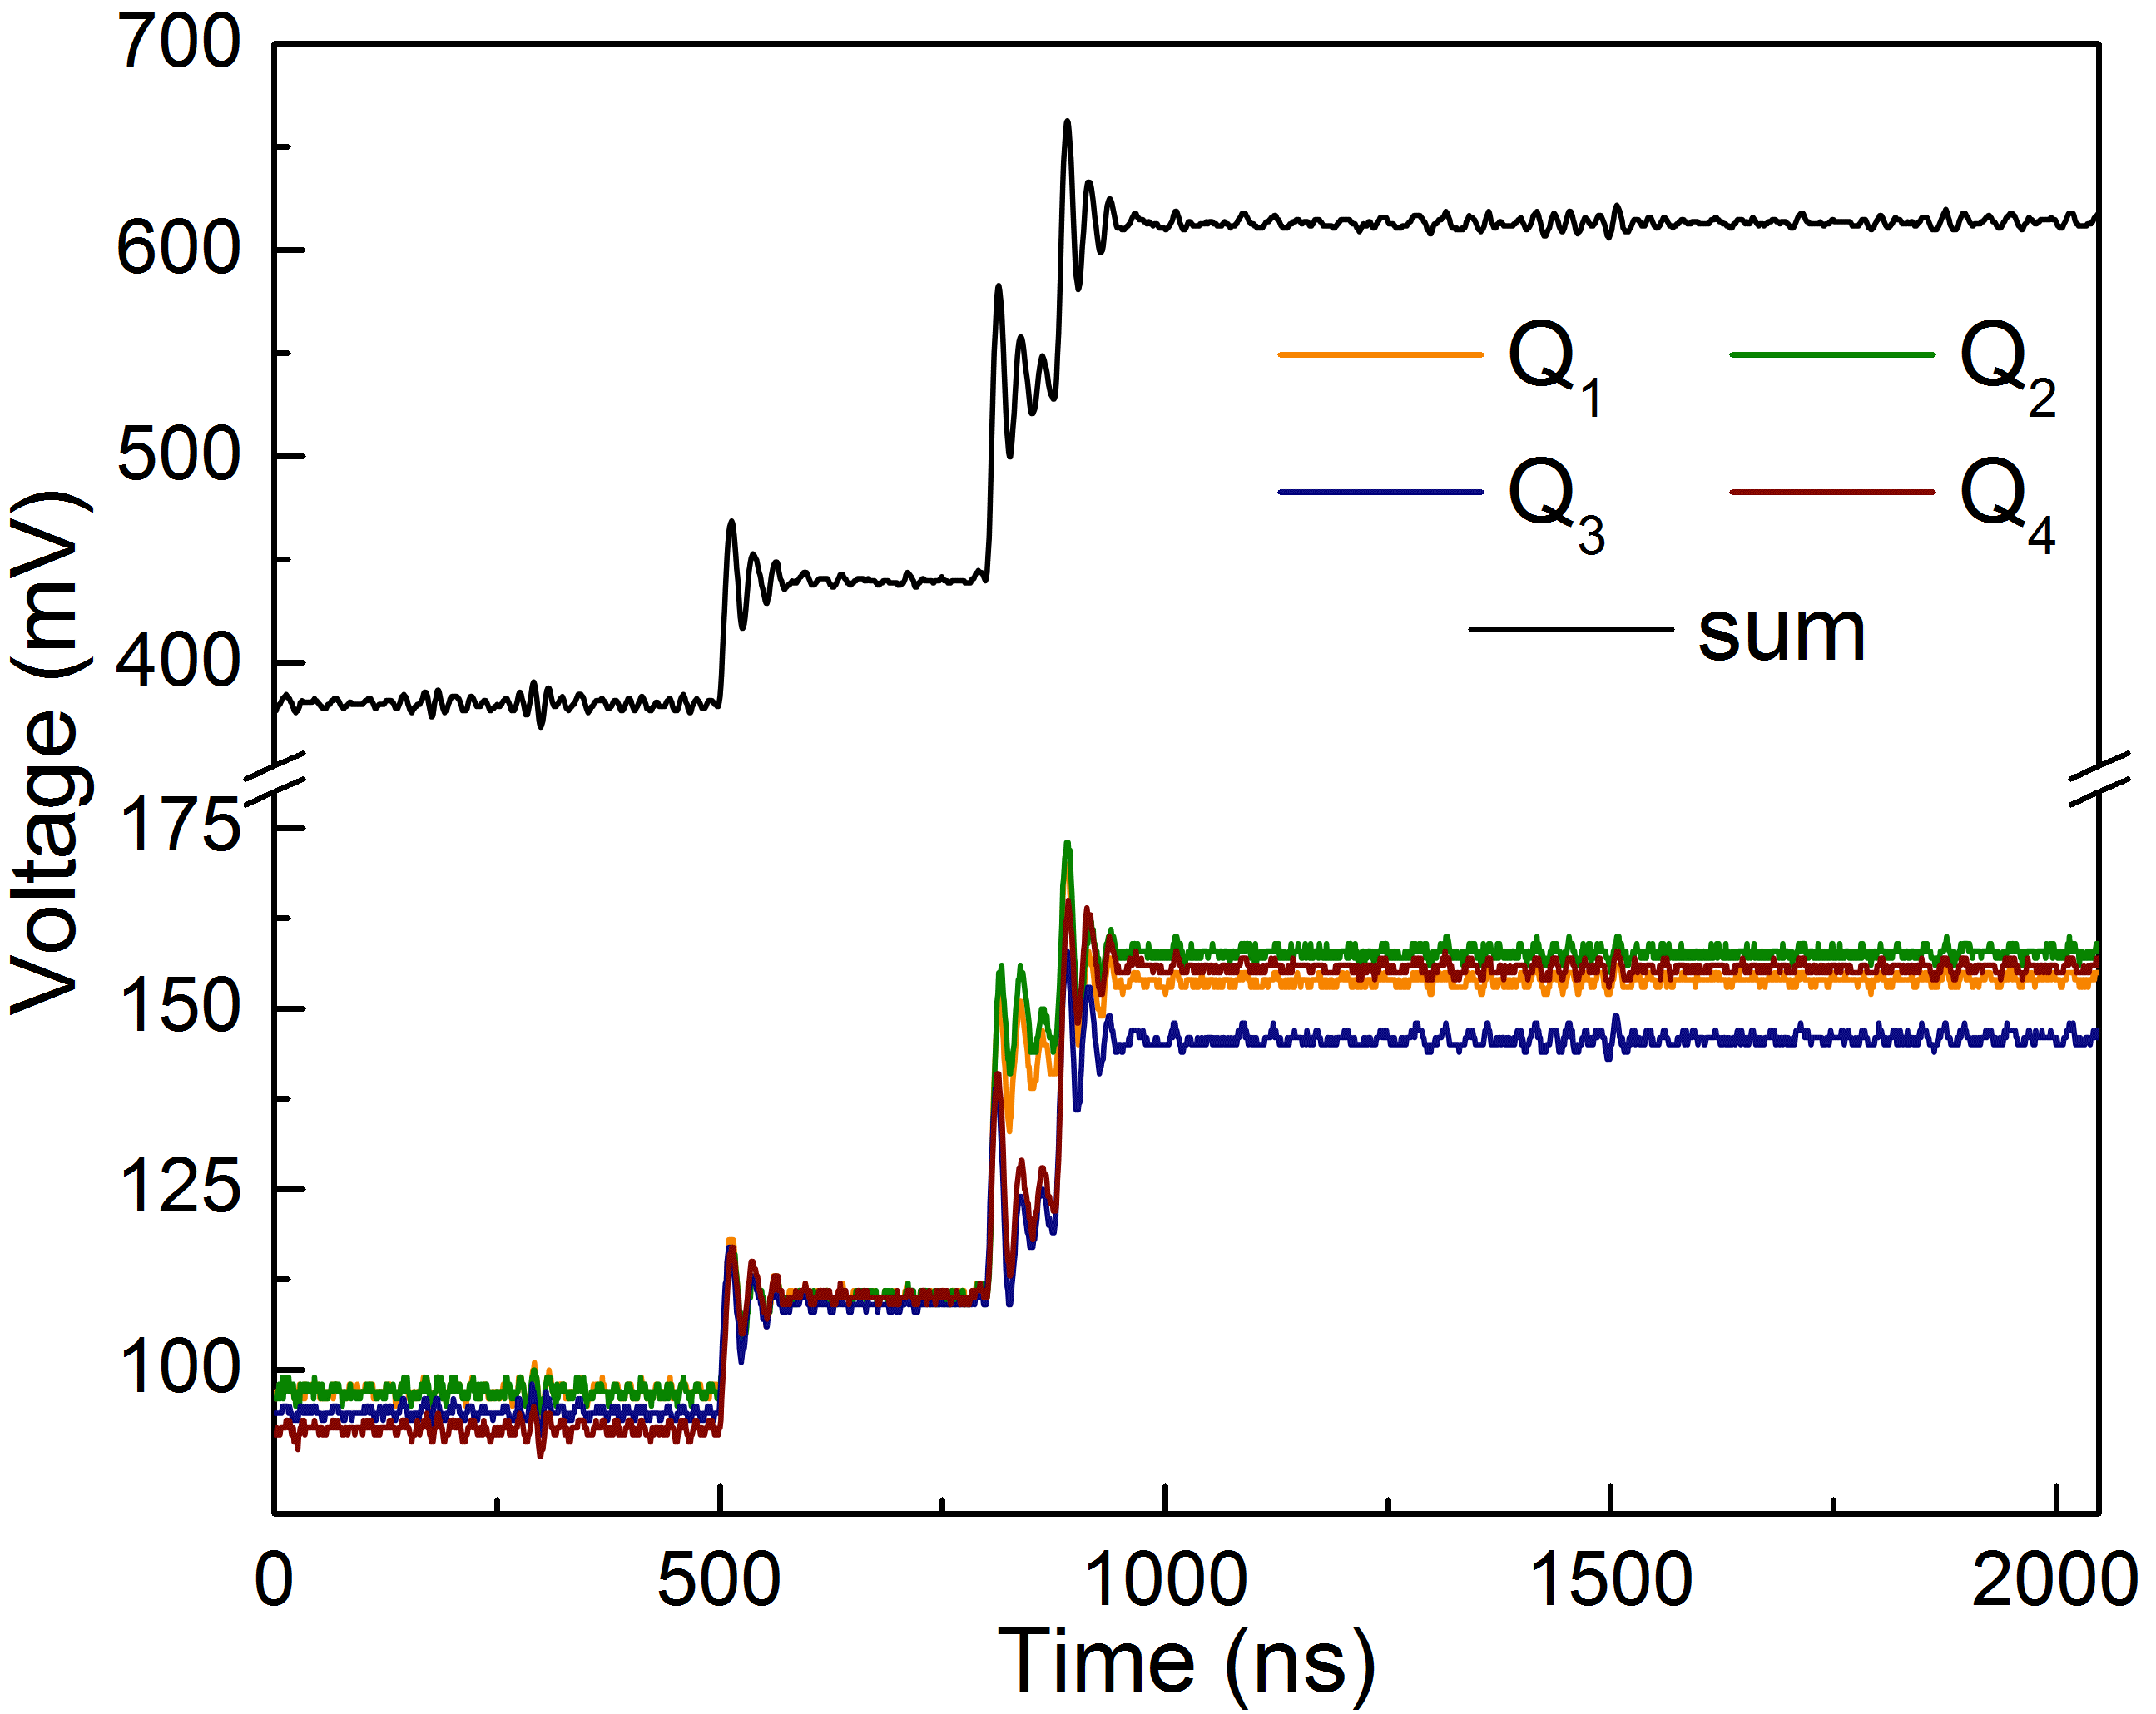
\includegraphics[width=\textwidth]{gfx/TripleCoincidenceEvent}
  \caption
  [Spectrometer response during a triple coincidence event.]
  {Spectrometer response during a triple coincidence event. This was taken during a CEI experiment studying the dynamics of \ch{CS2} at the Canadian Light Source. The fragmentation event showcased is the concerted breakup process \ch{CS2 $\rightarrow$ CS2^3+ $\rightarrow$ C^+ + S^+ + S^+}. As the carbon atom is lighter, the first step at \SI{500}{\ns} is the detection of the carbon atom. All four channels increase by roughly similar amounts hinting that the carbon atom was detected near the center of the detector by \eqref{eq:xy}. Then the second and third events belong to the two sulfur atoms, arriving later due to sulfur's larger atomic mass. If the molecule was aligned in a plane parallel to the detector, the two sulfur atoms would have remained at the same height throughout the Coulomb explosion and been detected at the same time, producing one step in the signal. However, it must have oriented vertically such that one sulfur atom was closer to the detector. During the Coulomb explosion, the closer atom will initially experience a kick towards the detector while the other sulfur atom will initially experience a kick away from the detector before being accelerated upwards due to the constant electric field. This results in one sulfur atom arriving earlier, and the other later. Looking at the individual signals, we see a significant increase in $Q_1$ and $Q_2$ at \SI{800}{\ns} suggesting that the first sulfur atom was on one side of the detector while the more significant increase in $Q_3$ and $Q_4$ at \SI{900}{\ns} suggest that the second sulfur atom was on the other side. This makes some intuitive sense as we expect the carbon atom to land somewhere near the middle and the two sulfurs to land on opposite sides of the detector. The oscilloscope cards sport an 8-bit bus and so the individual $Q_i$ channels were limited to \SI{200}{\mV} to increase position detection accuracy. I must admit that a nice and rich signal such as this one only makes up 1\% of all events, the majority being single or double coincidences.}
  \label{fig:tripleCoincidence}
\end{figure}

Software can analyze the signals and determine the magnitude of each $Q_i$ signal. If the change in baseline before and after an event is denoted $Q_i'$ then the position of the electron is then calculated using
\begin{equation}\label{eq:xy}
x = \frac{Q_1' + Q_2'}
         {Q_1' + Q_2' + Q_3' + Q_4'} ,\quad
y = \frac{Q_1' + Q_3'}
         {Q_1' + Q_2' + Q_3' + Q_4'}
\end{equation}
where $x,y \in [0,1]$ are fractional positions. Multiplying $x$ and $y$ by the dimensions of the MCP detector will yield the physical position of the cloud's centroid.

\subsection{Calculating the atomic fragments' momenta}
Calculating the momentum vector of each atomic fragment is an elementary physics problem once we have the time and position measurements. Let us look at the $p_x$ and $p_y$ components first.

The components of the three-dimensional momentum vector $\mathbf{p} = (p_x,p_y,p_z)$ for each atom are then calculated as

\begin{equation}\label{eq:CEImomenta}
p_x = \frac{m(x-x_0)}{t} ,\;
p_y = \frac{m(y-y_0)}{t} ,\;
p_z = \frac{qV}{2\ell} \left( \frac{t_0^2 - t^2}{t} \right)
\end{equation}
where $m$ is the atom's mass, $(x,y)$ is the location the atom collided with the MCP detector, and $(x_0,y_0)$ is the location that the Coulomb explosion originated. The location $(0,0)$ corresponds to the physical center of the MCP detector. $q$ is the net charge of the atom, $V$ is the value of constant electric potential the atom is subjected to, and $\ell$ is the distance from the location of the Coulomb explosion to the detector. $t$ is measured time of flight (between Coulomb explosion and detection) of the atom and 
\begin{equation}
t_0 = \sqrt{\frac{2d\ell}{V} \left( \frac{m}{q} \right)}
\end{equation}
is the atom's time of flight assuming no external forces act on it during its trip to the detector.

\subsection{Measurement uncertainty in the momenta}
For any relation $f = f(x_1, x_2, \dots, x_n)$, assuming independent variables, the absolute uncertainty in $f$, denoted $\Delta f$, may be calculated as
\begin{equation}
\Delta f = \sqrt{\sum_{i=1}^{n} \left( \frac{\partial f}{\partial x_i} \Delta x_i \right)^2}
\end{equation}
where $\Delta x_i$ is the uncertainty in the independent variable $x_i$.

Using this we may calculate the uncertainty in the measured momentum values, which will we different for each component. In our case, $p_x = p_x(m,x,x_0,t)$ and $p_y = p_y(m,y,y_0,t)$, however, the uncertainty in the atomic mass $m$ is orders of magnitude smaller than the uncertainty in the other variables and so we will ignore its effects. Thus we get that
\begin{subequations}
  \begin{align}
  \Delta p_x &= \sqrt{
    \left( \frac{\partial p_x}{\partial x}\Delta x \right)^2
    + \left( \frac{\partial p_x}{\partial x_0}\Delta x_0 \right)^2
    + \left(\frac{\partial p_x}{\partial t}\Delta t \right)^2
   } \\
  \Delta p_y &= \sqrt{
    \left( \frac{\partial p_y}{\partial y}\Delta y \right)^2
    + \left(\frac{\partial p_y}{\partial y_0}\Delta y_0 \right)^2
    + \left(\frac{\partial p_y}{\partial t}\Delta t \right)^2
  }
  \end{align}
\end{subequations}
where the partial derivatives can be calculated from \eqref{eq:CEImomenta} as
\begin{subequations}
  \begin{align}
  \frac{\partial p_x}{\partial x} = \frac{m}{t} &,\quad \frac{\partial p_x}{\partial x_0} = \frac{m}{t} ,\quad \frac{\partial p_x}{\partial t} = -m\frac{x-x_0}{t^2}\\
  \frac{\partial p_y}{\partial y} = \frac{m}{t} &,\quad \frac{\partial p_y}{\partial y_0} = \frac{m}{t} ,\quad \frac{\partial p_y}{\partial t} = -m\frac{y-y_0}{t^2}
  \end{align}
\end{subequations}
and so
\begin{subequations}
  \begin{align}
  \Delta p_x &= p_x \sqrt{
    \left( \frac{\Delta x}{x - x_0} \right)^2
    + \left( \frac{\Delta x_0}{x - x_0} \right)^2
    + \left( \frac{\Delta t}{t} \right)^2 } \\
  \Delta p_y &= p_y \sqrt{
    \left( \frac{\Delta y}{y - y_0} \right)^2
    + \left( \frac{\Delta y_0}{y - y_0} \right)^2
    + \left( \frac{\Delta t}{t} \right)^2 }
  \end{align}
\end{subequations}

Repeating the process for $p_z = p_z(q,V,\ell,t_0,t)$ but ignoring the tiny uncertainties in $q$, $V$, and $\ell$, we get
\begin{equation}
\Delta p_z = p_z \sqrt{
  \left( \frac{2tt_0}{t_0^2 - t^2} \Delta t_0 \right)^2
  + \left( \frac{t^2 + t_0^2}{t(t_0^2 - t^2)} \Delta t^2 \right)^2
}
\end{equation}

\section{Computationally simulating a Coulomb explosion} \label{sec:simulating}
To simulate an explosion of a molecule containing $n$ atoms, we must solve the classical equations of motion for each ion right after the explosion. We choose to use Hamiltonian mechanics here to acquire a system of first-order differential equations which may be easily solved by numerical methods such as the ubiquitous fourth-order Runge-Kutta. Assuming a purely electromagnetic potential for each ion, the Hamiltonian of the molecular system is
\begin{equation}
\mathcal{H}(\mathbf{r}_i, \mathbf{p}_i, t) = \sum_{i=1}^n \frac{\mathbf{p}_i^2}{2m_i} + \frac{1}{4\pi\epsilon_0}\sum_{\substack{\lbrace i,j\rbrace\\ i \ne j}} \frac{q_iq_j}{|\mathbf{r}_i-\mathbf{r}_j|}
\end{equation}
where $i,j \in \lbrace 1,2,\dots, n \rbrace$ and so the second summation is over all $i,j$ pairs where $i \ne j$. Calculating Hamilton's equations for the system, we get
\begin{subequations}
  \begin{align}
  \frac{d\mathbf{r}_i}{dt} &= \frac{\partial \mathcal{H}}{\partial \mathbf{p}_i} = \frac{\mathbf{p}_i}{m_i} \\
  \frac{d\mathbf{p}_i}{dt} &= \frac{\partial \mathcal{H}}{\partial \mathbf{r}_i} = \frac{1}{4\pi\epsilon_0}\sum_{j, \; j \ne i} \frac{\mathbf{r}_i - \mathbf{r}_j}{|\mathbf{r}_i - \mathbf{r}_j|^3}
  \end{align}
\end{subequations}
where $i$ is held fixed over the second summation. With appropriate initial conditions this system of $6n$ scalar first-order ordinary differential equations may be easily solved using, for example, the classical fourth-order Runge-Kutta method for numerically solving ordinary differential equations. The atoms are assumed to be at rest so that $\mathbf{p}_i(t=0) = 0$, while the initial positions, $\mathbf{r}_i(t=0) = 0$, are chosen to correspond to the molecular geometry. \footnote{Discuss the validity of the at rest assumption.}

One way to think of the problem being tackled in this thesis is: which initial geometry $\mathbf{r}_i(t=0) = 0$ results in the momentum values measured at the detector? The atoms are far enough apart after just a few nanoseconds that by the time they arrive at the detector, they feel almost no forces due to each other and their momenta attain asymptotic values which we can denote $\mathbf{p}_i(t\rightarrow\infty)$.

\section{Dimensionality reducing conventions for describing geometries and momenta} \label{sec:conventions}
While tackling the problem of geometry reconstruction, it will be crucial to choose a convention for describing the geometries and momentum vectors especially so that geometries and vector arrangements can be compared with ease. Even more importantly, it provides us with an opportunity to reduce the dimensionality of the problem from $3N$ to $3N-6$ for a molecular system with $N$ atoms. This stems from the fact that we only need to describe the relative position of each atom, not its absolute position. For example, a triatomic molecule can be described by two bond lengths and a bond angle, rather than three position vectors. Also, the exact same molecule can produce different momentum vectors after a Coulomb explosion depending on its initial orientation with respect to the detector. We must use a momentum convention to ensure a one-to-one mapping between geometries and measured momentum vectors.

\subsection{Triatomic molecules}
\subsection{Describing larger molecular geometries by a Z-matrix}
\subsection{A general convention for describing momentum vector arrangements}